\section{Problém password managerov}
Password manager ponúka používateľovi mnohé výhody a možnosti. Od generátora hesiel a ich automatického vyplnenia pri prihlasovaní do stránok, cez synchronizáciu medzi zariadeniami, zálohovanie, až po automatickú, pravidelnú zmenu jednotlivých hesiel. Napriek tomu existuje problém týchto managerov, ktorý ostal neriešený. Jemu sa bude táto kapitola venovať.

\subsection{Súčasný stav na trhu}
Ak hovoríme o heslách, priame (explicitné) používanie nižšie uvedených aplikácií pri dennom používaní je minimálne. A to vďaka automatickému vypĺňaniu hesla. Používateľ vstúpi na webovú stránku alebo do aplikácie. Pred vstupom sa musí prihlásiť do svojho účtu. Tam mu password manager výzvou ponúkne automatické vyplnenie (angl. výraz ,,autofill'') prihlasovacieho mena a hesla. Toto poskytuje vysokú úroveň komfortu. Používateľ nielen že nemusí vypisovať svoje prihlasovacie údaje manuálne, ale aj ich bezpečnosť porástla na vyššiu úroveň. Vďaka password manageru.
\par Podobne to funguje pri registrácii nového konta. Niektoré password manager aplikácie ponúknu náhodne vygenerované silné heslo (iCloud Keychain, \cite{10}). Používateľ sa môže rozhodnúť ho prijať. V takom prípade sa heslo pre vytvorený účet uloží do password manageru a ten ho pri každom ďalšom prihlásení vyplní. 
\subsubsection{LastPass} 
LastPass patrí medzi jeden z najpopulárnejších, čo sa týka počtu používateľov \cite{11}. Všetky heslá a ostatný obsah sú uzamknuté pod jedným master heslom. LastPass ale povoľuje aj vstup do jeho aplikácie pomocou biometrickej autentifikácie, ktorú väčšina smartfónov podporuje. Používateľ tak nemusí každý raz písať dlhé master heslo. Jediné, čo stačí, je priložiť prst, či pozrieť sa na smartfón (sken tváre). 
\par LastPass je client-server aplikácia. To znamená, že niektoré operácie a procesy prebiehajú na strane kienta, teda priamo v danom zariadení, ktoré používateľ drží a niektoré prebiehajú na strane LastPass serverov. Samotné šifrovanie, aj dešifrovanie prebieha na strane zariadenia \cite{12}. LastPass vytvorí kľúč z master hesla pomocou šifry AES (Advanced Encryption Standard) s hašovaním PBKDF2 (Key Derivation Function), SHA (Secure Hash Algorithm) s pridaným saltom \cite{13}. Týmto algoritmom sa bližšie venujeme v X.X (TODO číslo sekcie kde budem vysvetľovať AES princíp a hašovanie).
\par Dáta sú synchronizované pomocou serverov, čo umožňuje zálohovanie a synchronizáciu medzi zariadeniami. Dátový prenos po sieti je chránený pomocou TLS/SSL (\cite{14} sa bližšie venuje tomuto protokolu). LastPass v bezpečnosti pokračuje v možnosti dvojfaktorovej autorizácie a overovania na základe lokácie: kedykoľvek sa užívateľ prihlasuje do aplikácie z inej lokality, je vyzvaný prostredníctvom emailu s linkom, ktorý po otvorení overí používateľa ako verifikovaného. LastPass má mnoho možností, ako napríklad zdieľanie hesiel s iným LastPass účtom, generovanie hesiel s používateľom zvolenou dĺžkou a podmienkami, hodnotenie sily hesiel (systém usúdi, či je heslo dostatočne bezpečné), či import hesiel pomocou CSV súboru alebo iného password manageru.
\newline
\begin{figure}[ht]
  \centering
  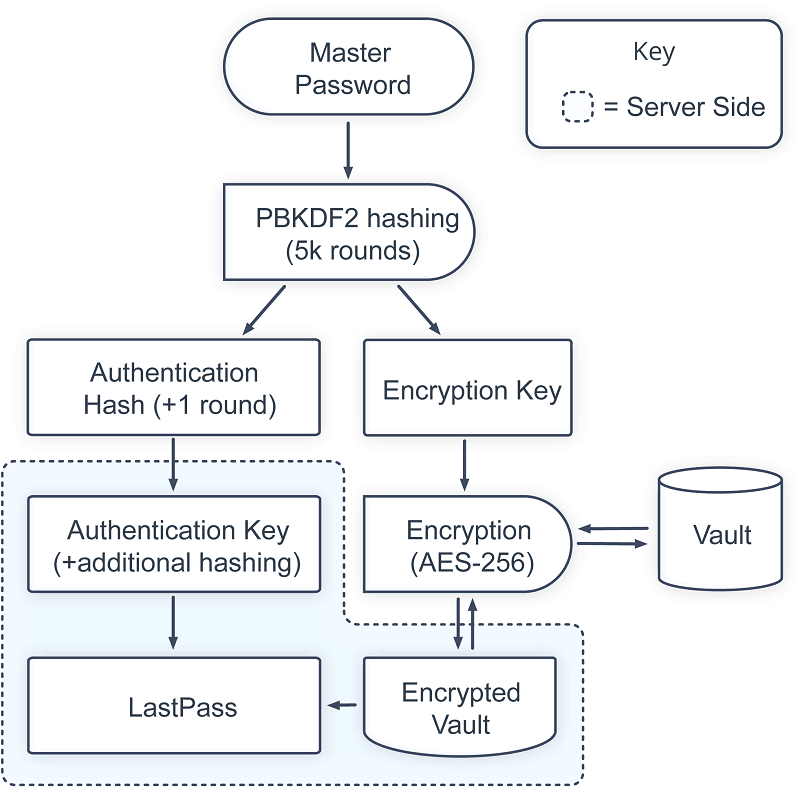
\includegraphics[width=8cm]{img/lastpass.png}
  \caption{Schéma šifrovania aplikácie LastPass.}
\end{figure}

\subsubsection{Dashlane}
Tento password manager je tiež vysoko využívaný \cite{15}. Jedna z jeho jedinečných funkcionalít je automatická zmena hesla \cite{16}. Používateľ si môže vybrať v zozname svojich hesiel, ktoré by sa mali automaticky meniť. Dashlane tak bude pravidelne generovať nové, komplexné heslá pre vybrané položky. Keďže medzi rôznymi webovými stránkami nie je jednotná architektúra a dizajn, nie všetky položky účtov vie Dashlane meniť automaticky. V takom prípade si užívateľ vie meniť heslo pre danú položku iba manuálne, v konkrétnej aplikácii alebo webovej stránke pre službu, ku ktorej prislúcha daný účet v Dashlane.
\par Tak ako LastPass, aj tento password manager dominuje silnou bezpečnosťou. Podporuje dvojfaktorovú autentifikáciu (dodatočné overenie po prvotnom prihlásení, viac v \cite{17}), šifru AES a synchronizáciu medzi zariadeniami. Mnohé z funkcionalít a možností má spoločné s aplikáciou LastPass. Nebudeme ich opäť spomínať, nakoľko cieľom tejto kapitoly je iba ukázať už existujúce vymoženosti rôznych password managerov.

\subsubsection{iCloud Keychain}
\par Za spomenutie určite stojí vstavaný password manager od spoločnosti Apple. Obsahuje určité funkcionality password managera, ktoré sú základnou súčasťou každého iOS, iPadOS, či MacOS zariadenia. Každý používateľ nejakého Apple zariadenia je identifikovaný pomocou AppleID konta. K nemu má pridelené cloud úložisko, kde sa mu všetky dáta zálohujú a synchronizujú so všetkými Apple zariadeniami.
\par Okrem fotiek, poznámok, kontaktov a iných dát tam sú uložené aj heslá z Keychainu. Keychain si pamätá nielen heslá, ale aj certifikáty, dôležité pri rôznych verifikáciach v rámci systému. Taktiež si pamätá kľúče. Sú verejné, ale aj súkromné, systém ich používa napríklad pri používaní iMessage (četovacia aplikácia). Sú šifrované pomocou šifry RSA a dĺžka kľúča je niekedy až 2048 bitov. \\

\par Z ostatných managerov ukážeme zopár ďalších funkcionalít, ktoré neboli spomenuté, respektíve ich LastPass, Dashlane, či Keychain neposkytujú.
\par 1Password ponúka takzvaný ,,Emergancy kit''. Po vytvorení 1Password účtu je používateľovi poskytnutý dokument. Následne je vyzvaný, aby si ho vytlačil, prípadne uložil na pamäťové médium. Dokument obsahuje prihlasovacie údaje a master heslo. Taktiež obsahuje QR kód, ktorý automaticky vyplní tieto dáta pri núdzovom prihlasovaní. \\

\begin{figure}[ht]
  \centering
  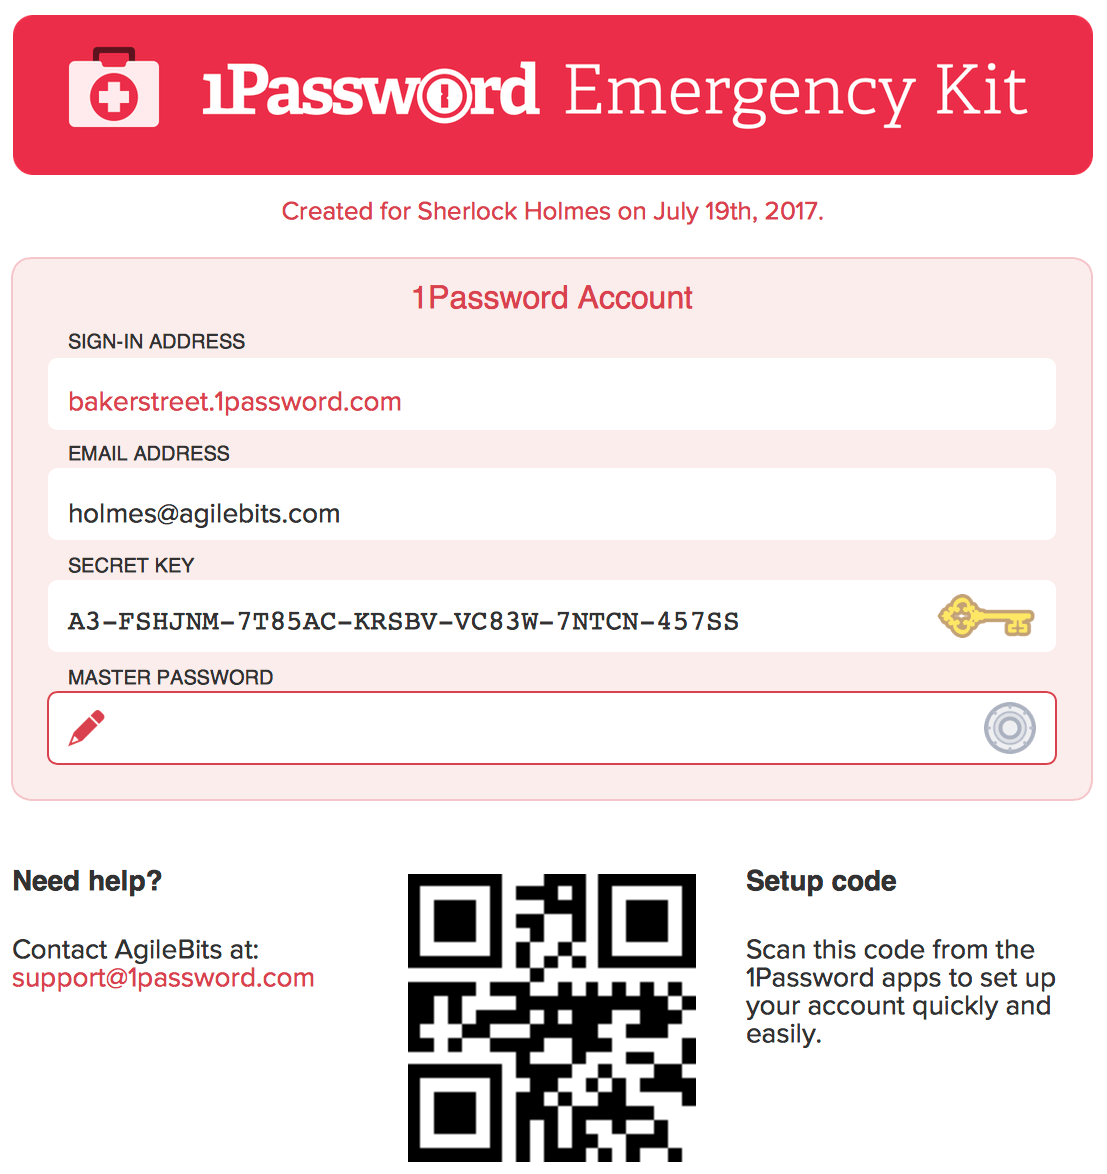
\includegraphics[width=8cm]{img/1pass.png}
  \caption{Emergency kit od 1Password - ukážka pdf súboru, ktorý používateľ obdrží.}
\end{figure}

\par Password manager Remembear ponúka jednoduchú aktiváciu aplikácie na novom zariadení prostredníctvom QR kódu. Za spomenutie stojí aj menej známy správca, konkrétne Myki. \par Myki ako jeden z mála nepoužíva svoje servery na zálohovanie a ukladanie hesiel. Namiesto toho využíva server iba ako sprostredkovateľa \cite{18} spojenia keď nastáva synchronizácia medzi zariadeniami. Teda, používať Myki na viacerých zariadeniach je akousi formou ,,zálohy''.
\par Vyššie spomenuté aplikácie fungujú na rôznych platformách: verzia pre smartfóny (iOS, Android), počítače (Windows, MacOS, Linux), inteligentné hodinky a podobne.
\subsection{Nízka popularita password managerov a nesprávne alternatívne spôsoby ukladania hesiel}
Ľahko sme vedeli ukázať, že bohatosť a rôznorodosť trhu s aplikáciami na správu hesiel je naozaj veľká. Používateľ by teda nemal mať problém vybrať si takú aplikáciu, ktorá vyhovuje jeho požiadavkám. Napriek tomu je popularita password managerov nízka. 
\par Už nadpis článku \cite{19} začína slovami \textit{,,Hardly Anybody Uses a Password Manager''}. Teda v slovenskom znení - ,,Horko-ťažko niekto vôbec používa password manager''. Píše o prieskume na túto tému a jeho výsledkoch. V Spojených štátoch a v Anglicku sa pýtali 1000 respondentov rôzne otázky. Týkali sa bezpečnosti pri používaní internetu. Išlo najmä o praktiky pri používaní hesiel; či pre každú stránku používajú iné heslo, či je heslo silné, dlhé alebo krátke, ,,náhodné'' alebo ľahko zapamätateľné. Spomedzi opýtaných, 59\% uviedlo, že používa 5 alebo menej rôznych hesiel, ktoré si pamätajú v hlave. Pritom 74\% sa denne prihlási do 6 a viac účtov. Môžeme už teraz hovoriť o pravdepodobnosti faktu, že niektorí z týchto používateľov používajú rovnaké heslo pre rôzne účty. Túto skutočnosť využívajú útočníci. Ak získajú heslo k jednému účtu, predpokladajú, že ho používateľ využíva aj v iných účtoch. Najmä, ak je heslo jednoduché. A ak hovoríme o respondentoch, ktorí si dokážu pamätať až do 5 hesiel v hlave a používajú ich na prihlasovanie do aspoň šiestich účtov, je veľmi pravdepodobné, že nie sú náročné (ani z hľadiska zapamätateľnosti, ani z hľadiska kryptografie).
\par Ďalšia negatívna skutočnosť, ktorá vyplýva z prieskumu je písanie hesiel na papier. Až 42\% opýtaných používa túto metódu. Niekto by argumentoval, že rovnako ako papier s heslami vie niekto ukradnúť aj server, kde sú uložené heslá password manageru. Aj keď sa môže zdať, že princíp je ten istý, na rozdiel od papiera s ručne vypísanými heslami sú heslá na serveroch password managerov zašifrované. Dnešné moderné šifry, ktoré sa na ich zašifrovanie používajú sú matematicky silné a v súčasnosti neprelomiteľné. Tá ťažšia časť je ukryť kľúč tak, aby ho nikto nenašiel. Dôvodom úspešných útokov teda nie je nedokonalosť moderných šifier. Väčšinou ide o postranné kanály, zlé ukrytie kľúča, spiknutie zvnútra a podobne.
\par Keď máme hovoriť o popularite password managerov, tento prieskum silno podporuje nadpis tejto podkapitoly. Len 8\% opýtaných používa na svoje heslá nejakého správcu. Naopak, jemne menej než tri štvrtiny si vystačí s tým, že si ich heslá zapamätá prehliadač. Tu treba uviesť skutočnosť, že ukladanie hesiel do prehliadača je náchylné na krádež pomocou malvéru (škodlivý softvér, ktorý sa snaží infikovať zariadenie, väčšinou využívaný na krádež citlivých údajov, najmä hesiel \cite{20}). 
\par Populárny prehliadač Google Chrome ponúka používateľovi možnosť zapamätať si heslá pri prihlasovaní na rôznych stránkach. Tieto heslá sú synchronizované do všetkých zariadení pomocou Google konta. Je ľahké sa dostať do tohto trezoru, stačí do URL text-boxu prehliadača napísať ,,chrome://settings/passwords'' \cite{21}. Zobrazí sa zoznam hesiel pre dané stránky, ktoré si prehliadač ukladal. Jedným tlačidlom sa odokryje heslo ako otvorený text. Chrome nevyžaduje žiadnu autentizáciu. Je jednoduché pre útočníka pri fyzickom prístupe k zariadeniu tieto dáta získať pár klikmi. Chrome vývojár Justin Schuh avšak argumentuje \cite{21}. Hovorí, že keď má niekto prístup do účtu operačného systému používateľa, vie, vidí a má prístup ku všetkému. Môžeme z tohto tvrdenia vyvodiť záver, že Chrome nevidí zmysel v chránení trezoru prehliadača (okrem hesla do Googlu účtu), lebo rozumie faktu, že ten, kto má prístup do operačného systému, má aj tak prístup ku všetkému.
\par Mozilla Firefox tiež nechráni svoj trezor hesiel, avšak narozdiel od Chromu ponúka aktiváciu master hesla. Spomeňme ešte Safari od Apple, ktorý chráni celý trezor heslom účtu operačného systému. Z výroku Schuha vyplýva, že takéto zabezpečenie je zbytočné. Apple pravdepodobne počíta s tým, že môže prísť k zneužitiu zariadenia už po prihlásení do systému, teda útočník nemusí poznať heslo. V takom prípade považujeme takéto zabezpečenie za múdre, avšak určite existujú bezpečnejšie spôsoby (za cenu komfortu).
\par Spomínaný prieskum z roku 2015 nepriniesol pozitívne výsledky. O tri roky neskôr sa uskutočnil ďalší \cite{22}. Spomedzi 2500 Američanov si 35\% nikdy heslá nemení. Robí tak iba po vyzvaní. Veľkým prekvapením bolo 11\% používateľov, ktorí si ich menia každý deň. The National Institute of Standards and Technology radí používateľom, aby si heslá menili nie pravidelne, ale až keď nastane ich prelomenie. Keď padla otázka, aký nástroj respondenti používajú na svoju ochranu na internete, víťazom bol antivírový software (53\%), password manager získal 24\%, čo je trojnásobný nárast za obdobie troch rokov\footnote{vychádzajúc zo vzorky opýtaných, teda určitá štatistická odchylka je pri týhto úvahách samozrejmosťou.}.
\par Napriek pozitívnemu nárastu popularity password managerov považujeme 24\% za malé číslo. Je pravdou, že tieto aplikácie sú na trhu nie tak dlho. Antivírový softvér má v tomto časový náskok. Tento softvér má avšak iný cieľ a zameranie v bezpečnosti, než password manager. Bolo by nezmyselné tieto dva nástroje na bezpečnosť porovnávať ako dve technologické riešenia, ktoré slúžia na rovnaký účel. U niektorých čitateľov možno vzniká otázka typu: \textit{Prečo používatelia nepoužívajú viac bezpečnostné nástroje na ochranu ich osobných údajov?} V druhom spomínanom prieskume z roku 2018 sa opýtaných pýtali aj na otázku, kedy boli poučení, respektíve vzdelaní na tému bezpečnosti na internete. Až 36\% nedostalo na túto tému žiadne vzdelanie. Aj toto môže byť odpoveďou na vyššie spomínanú otázku.
\par Ďalším dôvodom môže byť nedôvera. Používatelia nemusia byť presvedčení o tom, že password manager naozaj ich heslá ochráni, nezverejní, prípadne nezneužije. Jedna práca \cite{23} študovala, prečo má password manager stále málo používateľov. Urobila prieskum, kde prizvala 137 respondentov používajúcich password manager a 111 takých, ktorí ho nepoužívajú. Vznikla štúdia, ktorá porovnáva odpovede na 6 otázok týchto dvoch skupín a snaží sa vyvodiť záver, prečo je popularita týchto aplikácií taká, aká je.

\section{Recitácia}
Citujem všetky zdroje v \textbf{bibliography.bib}, \cite{t00, t01, t02, t03, kniha, kniha2, kniha3, small, big, cs, koll, kap, tug, knuth, zbornik, prispevok}. \newline Good luck.
\section{Možnosti anonymizácie}
\noindent Anonymizácia znamená zmena alebo úprava údajov tak, aby sa podľa nich nedala jednoznačne určiť osoba, ktorej tieto údaje patria \cite{t01}. Existuje niekoľko spôsobov, ktorými môžeme dosiahnuť rôznu úroveň anonymizácie na internete: od mazania cookies súborov po ukončení prehliadania webových stránok až po používanie operačných systémov, ktoré sú na anonymite založené; od bezplatných možností až po komerčné verzie.  
\newline Nasleduje priblíženie niektorých možnosti anonymizácie.

\subsection{Súkromné prehliadanie}
\noindent Najpoužívanejšie internetové prehliadače súčasnosti majú v sebe zabudovanú funkcionalitu, ktorá dokáže čiastočne anonymizovať prístup na internet. Táto funkcionalita blokuje ukladanie navštívených stránok do histórie a nezaznamenáva súbory, ktoré sa stiahnu z~internetu. \acrshort{sw} a \acrlong{hw} sú skratky.

\begin{table}[!htbp]
\caption{Moduly a ich funkcie pri anonymizácii}
\label{modulyVlastnosti}
\begin{center}
\begin{tabular}{p{4cm}|c|c|c|c|c|c|c|c|c|c|c|c|c|c|c}
& \multicolumn{14}{c}%
	 {\textbf{Funkcia}}\\ \hline
&&&& & &\multicolumn{8}{c}%
	 {Modifikácia}\\ 
\textbf{Modul} &\begin{sideways} zobrazenie hlavičky \end{sideways} &\begin{sideways} blokovanie skriptov \end{sideways} &\begin{sideways} zmena IP \end{sideways} & \begin{sideways} zmena lokalizácie \end{sideways} & \begin{sideways} zmazanie/blokovanie cookies \end{sideways} & \begin{sideways} blokovanie trackerov \end{sideways}  & \begin{sideways} popis \end{sideways} & \begin{sideways}používateľský agent\end{sideways} & \begin{sideways} kódové označenie prehliadača \end{sideways} & \begin{sideways} názov prehliadača \end{sideways} & \begin{sideways} verzia prehliadača \end{sideways} & \begin{sideways} platforma \end{sideways} & \begin{sideways} výrobca prehliadača \end{sideways} & \begin{sideways} označenie výrobcu prehliadača \end{sideways} \\ \hline
User agent switcher & & & & & &  & X & X & X & X & X & X & X & X  \\ \hline
Ghostery &  && & & X & X &  &  & & & & & & \\  \hline
Better privacy && &  & & X &  &  &  & & & & & & \\  \hline
Anonymox &  && X & X & X &  & X & X & & & & & & \\  \hline
Modify headers & & &  &  & X &  &  & X &  &  &  & & &  \\  \hline
Request policy & & &  &  & & X  &  &  &  &  &  & & &   \\  \hline
Live HTTP headers & X& &  &  & &  &  &  &  &  &  & & &   \\  \hline
User agent awitcher for chrome & & &  &  & &  & X & X &  &  &  & & &   \\  \hline
Header hacker & & &  &  & &  & X & X & X & X & X & X & X & X    \\  \hline
Mod header & & &  &  & &  & X & X & X & X & X & X & X & X    \\  \hline
Script no & &X &  &  & &  &  &  &  &  &  &  &  &     \\  \hline
No script & &X &  &  & &  &  &  &  &  &  &  &  &     \\  \hline
Proxify it & & &X  & X & &  &  &  &  &  &  &  &  &     \\  \hline
I'm not here & & &  & X & &  &  &  &  &  &  &  &  &     \\  \hline
Get anonymous personal edition & &X &X &X &X&X &  &  &  &  &  &  &  &     \\  \hline
Anonymous browsing toolbar & & & X & X & &  &  &  &  &  &  &  &  &     \\  \hline
Easy hide your IP and surf anonymously & & & X & X& &  &  & X & X & X & X &  &  &     \\  \hline
\end{tabular}
\end{center}
\end{table}

\subsection{Anonymná sieť}
\noindent Anonymná sieť je sieť serverov, medzi ktorými dáta prechádzajú šifrované. V anonymných sieťach dáta prechádzajú z počítača používateľa, odkiaľ bola požiadavka poslaná, cez viaceré proxy smerovače, z ktorých každý správu doplní o smerovanie a zašifruje vlastným kľúčom. Cesta od ...


\subsection{Funkcionalita}
\noindent  Rozšírenie tiež okrem splnenia špecifikácie malo pre prehľadnosť a overenie funkčnosti zobrazovať údaje, ktoré boli na server odoslané. Zoznam údajov odoslaných na server, sa mal ukladať do krátkodobej histórie, aby nemal používateľ k dispozícií len najnovšie údaje, ale aj údaje odoslané v nejakom časovom období. Nejaky listing z priloh \ref{lst:sublime}.

\subsubsection{Funkcionalita2}
\noindent Samozrejmosťou bolo nastavenie zapnutia rozšírenia pri štarte, prípadne interval zmeny odosielaných údajov.

\subsection{Vzhľad}
\noindent Dôležitou požiadavkou kladenou na rozšírenie bolo príjemné používateľské rozhranie. Z~tohto dôvodu malo rozšírenie obsahovať zoznam modifikovaných vlastností a tlačidlo pre prístup k nastaveniam rozšírenia v jednoduchej a praktickej forme. Predpokladaný vzhľad je zobrazený na obrázku č. \ref{vzhladobr}.
\begin{figure}[!htbp]
  \centering
  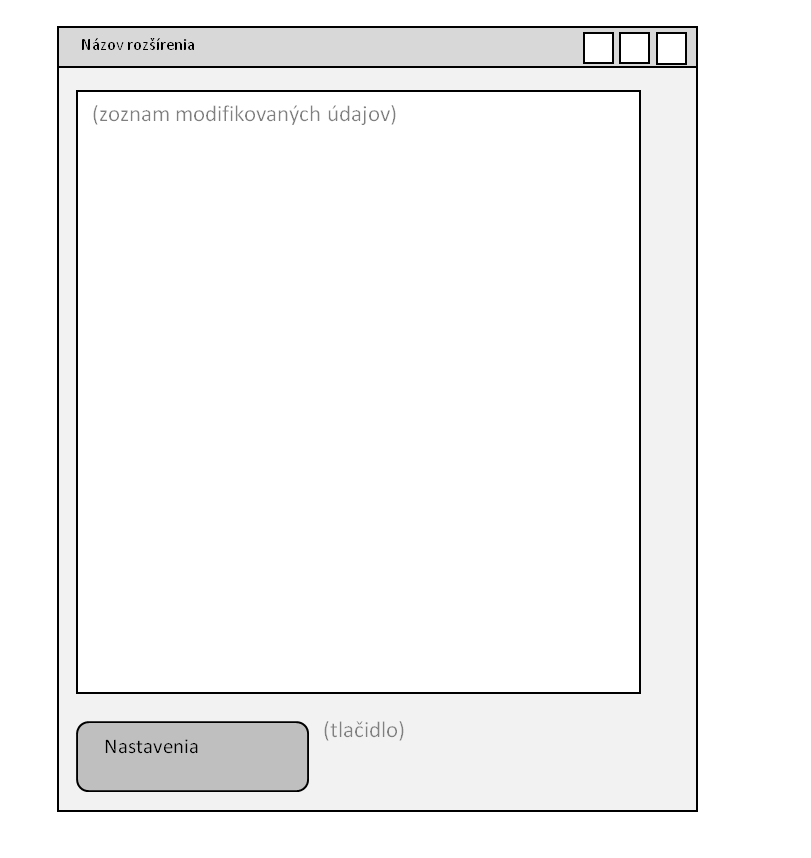
\includegraphics[width=8cm]{img/vzhlad.png}
  \caption{Predpokladaný vzhľad rozšírenia.}
  \label{vzhladobr}
\end{figure}	 
\noindent Dôležitou požiadavkou kladenou na rozšírenie bolo príjemné používateľské rozhranie.\cite{t00} Z~tohto dôvodu malo rozšírenie obsahovať zoznam modifikovaných vlastností a tlačidlo pre prístup k nastaveniam rozšírenia v jednoduchej a praktickej forme. Predpokladaný vzhľad je zobrazený na obrázku č. \ref{vzhladobr}.

\begin{algorithm}
\scriptsize
\begin{algorithmic}
 \STATE <text>
 \IF{<condition>} \STATE {<text>} \ELSE \STATE{<text>} \ENDIF
 \IF{<condition>} \STATE {<text>} \ELSIF{<condition>} \STATE{<text>} \ENDIF
 \FOR{<condition>} \STATE {<text>} \ENDFOR
 \FOR{<condition> \TO <condition> } \STATE {<text>} \ENDFOR
 \FORALL{<condition>} \STATE{<text>} \ENDFOR
 \WHILE{<condition>} \STATE{<text>} \ENDWHILE
 \REPEAT \STATE{<text>} \UNTIL{<condition>}
 \LOOP \STATE{<text>} \ENDLOOP
 \REQUIRE <text>
 \ENSURE <text>
 \RETURN <text>
 \PRINT <text>
 \COMMENT{<text>}
 \AND, \OR, \XOR, \NOT, \TO, \TRUE, \FALSE
\end{algorithmic}
\caption{Ukážka príkazov pre algorithmic}  
\label{alg:preview}  
\end{algorithm}

\begin{lstlisting}[
  caption={Ukážka algoritmu},
  label={lst:main-c},
  language=c
]
/* Hello World program */

#include<stdio.h>

struct cpu_info {
    long unsigned utime, ntime, stime, itime;
    long unsigned iowtime, irqtime, sirqtime;
};

main()
{
    printf("Hello World");
}
\end{lstlisting}